
\chapter{Error Correction in a Non-Abelian Topologically Ordered System}

The work in this chapter is based on the collaboration \cite{Burton2015}.

In this chapter we apply the methods of Chapter 3 
to develop a simulation of noise processes in a two dimensional
system with non-abelian anyons.

Topologically ordered quantum systems in two dimensions show great promise for 
long-term storage and processing of 
quantum information~\cite{Kitaev2003, Dennis2002, Nayak2008}. 
The topological features of such systems are insensitive to local 
perturbations~\cite{Bravyi2010, Bravyi2011a, Michalakis2013}, and they
have quasiparticle excitations exhibiting anyonic
statistics~\cite{Wilczek1990}. These systems can be used as
quantum memories~\cite{Kitaev2003, Dennis2002} or to
perform universal topological
quantum computation~\cite{Freedman2002, Nayak2008}.

Quantum error correction is vital
to harnessing the computational power of topologically
ordered systems. When coupled to
a heat bath at any non-zero temperature, thermal fluctuations
will create spurious anyons that diffuse and quickly corrupt the stored quantum 
information~\cite{Pastawski2010}. Thus, the passive protection provided by the mass gap
at low temperature must be augmented by an \emph{active} decoding procedure. 

In order to efficiently classically simulate an error-correction protocol for
a topologically ordered quantum memory, it is necessary to simulate  
the physical noise processes, the decoding algorithm, and the physical recovery operations.
Decoding algorithms are typically designed to run efficiently on a 
classical computer, but there is generally no guarantee that the  
noise and recovery processes should be classically simulable.
Because of this, almost all of the sizable research effort 
on active quantum error correction for topological systems has focused
on the case of abelian
anyons~\cite{Dennis2002, Duclos-Cianci2010, Duclos-Cianci2010a, Wang2010, Wang2010a,
Duclos-Cianci2013, Bravyi2011, Bombin2012, Wootton2012, Anwar2014,
Watson2014, Hutter2014a, Bravyi2014, Wootton2015, Fowler2015,
Andrist2015}, which can be efficiently
simulated due to the fact that they cannot be used for quantum computation.
%Systems of abelian anyons are well suited to studying quantum 
%error correction because (at the RG fixed point) noise and 
%recovery processes can be efficiently simulated numerically, allowing lattice simulations 
%of decoding with over 1 million sites~\cite{Duclos-Cianci2010}. 
%Standard algorithms are specifically tailored to exploit the abelian nature 
%of these particles,
%particularly that abelian anyons cannot be used for quantum computation. 

Recent investigations have begun to
explore quantum error correction for non-abelian anyon
models~\cite{Brell2013, Wootton2013, Hutter2014, Wootton2015b, Hutter2015continuous}.
Nonabelian anyon models are especially interesting 
because braiding and fusion of
these anyons in general allows for the implementation of universal quantum 
computation. However, the initial studies
of error-correction in non-abelian anyon
systems have focused on specific models, such as the Ising 
anyons~\cite{Brell2013, Hutter2015continuous} and the so-called $\Phi$-$\Lambda$
model~\cite{Wootton2013, Hutter2014} that, while non-abelian,
are not universal for quantum
computation. The general dynamics of
these particular anyon models is
known to be efficiently classically simulable, a fact
that was exploited to enable efficient simulation of error correction
in these systems. When considering more general anyon models, their 
ability to perform universal quantum computation would seem a significant
barrier to their simulation on a classical computer. While simulation 
of general dynamics does indeed seem intractable, we argue that 
the kinds of processes that are typical of thermal noise 
are sufficiently structured  to allow for their classical simulation
in the regimes where we expect successful error correction to
be possible. This insight allows us to simulate the noise
and recovery processes for a quantum code based on a universal anyon model.

Concretely, we consider quantum error correction in a two-dimensional
system with Fibonacci anyons, a class of non-abelian anyons that are universal for quantum
computation~\cite{Freedman2002, Nayak2008}. Fibonacci anyons are
experimentally motivated as the
expected excitations of the $\nu=\frac{12}{5}$ fractional quantum Hall
states~\cite{Slingerland2001}, and can be realized in several spin
models~\cite{Levin2005, Bonesteel2012, Kapit2013, Palumbo2014} and composite
heterostructures~\cite{Mong2014}.
Any of these physical systems
could be used to perform
universal topological quantum computation, and
can be modelled by our
simulations. Natural sources of noise
from thermal fluctuations or external
perturbations will be suppressed by
the energy gap but must still be corrected to allow for scalable computation.

We use a flexible phenomenological model of dynamics and thermal
noise to describe a system with Fibonacci anyon excitations. Within
this model, we apply existing general topological error-correction protocols, and
simulate the successful preservation of quantum information encoded in topological
degrees of freedom. Topological quantum computation protocols using non-abelian anyons
typically implicitly assume the existence of an error-correction protocol to
correct for diffusion or unwanted creation of anyons.
The ability to simulate the details of how and when
these techniques succeed on finite
system sizes has not previously
been available, and so our
results are the first explicit
demonstration that such a scheme
will be successful when applied
to a universal topological quantum computer.

%%%%%%%%%%%%%%%%%%%%%%%%%%%%%%%%%%%%%%%%%%%%%%%%%%%%%%%%%%%%%%%%%%%%%%%%%%%%%%%
%
%

\section{Fibonacci anyons}

The defining difference between abelian and non-abelian
anyon theories is that in
an abelian theory particle content
alone uniquely determines the outcome
of joint charge measurements.
In
contrast, outcomes for non-abelian charge
measurements depend on the history
of the particles as well
as their type.
We consider a system supporting non-abelian Fibonacci
anyon excitations, denoted by $\tau$.
Two such anyons can have total charge
that is either $\tau$ or $\vac$ (vacuum), or any superposition of these, and
so the fusion space in this case is 2-dimensional.

For Fibonacci anyons, the non-trivial $R$ and $F$ moves are
\begin{equation*}
        R_{\vac}^{\tau\tau} = \e^{\frac{-4\pi i}{5}} 
        \ \ , \ \
        R_\tau^{\tau\tau}= \e^{\frac{3\pi i}{5}} 
        \ \ , \ \
        F_{\tau}^{\tau\tau\tau} = \begin{pmatrix}\phi^{-1}&\phi^{-\frac{1}{2}}\\\phi^{-\frac{1}{2}}&-\phi^{-1}\end{pmatrix} \,,
\end{equation*}
where the matrix is given in a
basis labelled $(\vac,\tau)$ and 
$ \phi=\frac{1+\sqrt{5}}{2} $
is the golden ratio.

In terms of skeins we write the F-moves as:
\begin{align*}
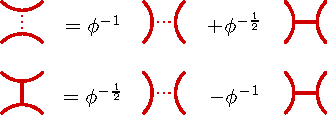
\includegraphics[]{pic-skein1.pdf}
\end{align*}
The solid lines represent Fibonacci world-lines.
The dotted lines represent vacuum charges,
and we are free to include these lines or not.
We leave these anyon paths
as undirected because Fibonacci anyons are
self-inverse.
The non-trivial $R$-moves are:
\begin{align*}
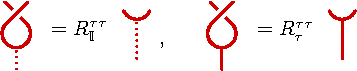
\includegraphics[]{pic-skein2.pdf}
\end{align*}

For more details of the Fibonacci anyon
theory, see e.g.\ Ref.~\cite{Nayak2008} and references therein.

%In addition to the fusion space there is also a
%global degeneracy associated with the topology of the
%manifold on which the anyons reside.
%We consider systems on a torus,
%which for the Fibonacci anyons gives rise to a 2-fold degeneracy.
%This extra degree of freedom can be thought of being
%associated with the total anyonic charge (or flux) running through
%the torus itself. Since there are two different possible charges
%in the Fibonacci anyon model, the global degeneracy is 2.


%%%%%%%%%%%%%%%%%%%%%%%%%%%%%%%%%%%%%%%%%%%%%%%%%%%%%%%%%%%%%%%%%%%%%%%%%%%%%%%
%
%

\section{Physical model}

\begin{figure}
\begin{center}
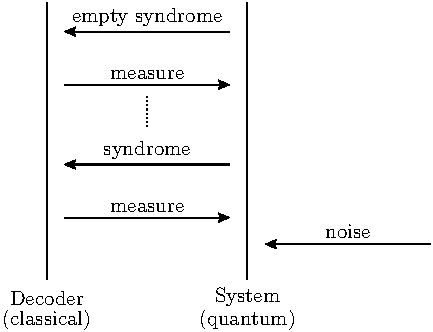
\includegraphics[]{pic-process.pdf}
\end{center}
\caption{
The simulation of a single round of
error correction involves two components: 
the classical decoder, and the quantum system.
After the noise process has been applied to the
system, the simulation proceeds as a dialogue between
the decoder and the system. 
Decoding is successful when all charges have been eliminated,
resulting in an empty syndrome.
}
\label{PicProcess}
\end{figure}

%\danbrowne{Clarify this with a figure. In chapter 3 you have only considered surfaces with boundary. How is a logical qubit encoded on a surface with no boundary?  Why is there a single qubit here (and not a higher number)?  How are logical operations implemented in this model? Important to introduce the logical operators that will form your logical errors.  Why did you choose this qubit encoding?}

We consider encoding quantum information in the fusion space of a torus.
As we saw in the previous chapter, 
the dimension of this space is equal to the number of
charges (the cardinality of $\mathcal{A}$).
For Fibonacci anyons, we have two charges, $\vac$ and $\tau$,
so this gives a fusion space equal to one qubit.
In this work we do not consider the logical operators that
act on the encoded state, but merely note that it is sufficient
to protect the state if all operations remain local.
\footnote{For an example of a \emph{non-local} operation we
create a pair of charges and take one of the charges around
a non-contractible loop of the torus.}

We endow the torus with an $L\times L$ square lattice of observables
\footnote{We defined the observables associated to a modular functor in section 3.3.}:
%\danbrowne{Add a link to refer back to the section in chapter 3 where you introduced observables. }
$$
    \Lambda := \bigl\{ \gamma_{ij} \bigr\}_{i,j=1,...,L}
$$
These observables are the physically accessible observables of
the noise reduction procedure we call the \emph{decoder.}
We call each such $\gamma_{ij}$ a \emph{tile.}
In the diagrams below 
there is a small gap between the tiles but this is not meant
to reflect an actual physical gap.
\begin{center}
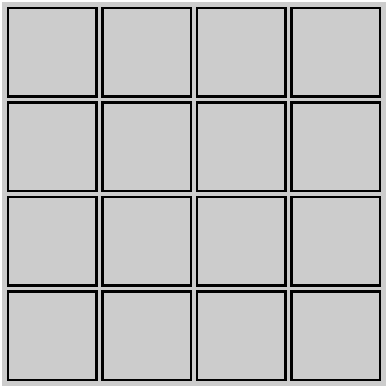
\includegraphics[width=0.3\columnwidth ]{pic-torus-tiles.pdf}
\end{center}

We also use these observables to construct an
idealized Hamiltonian of the form
$H = -\sum_{\gamma\in\Lambda} \ket{\vac}\bra{\vac}_\gamma,$
where $\ket{\vac}\bra{\vac}_\gamma$ is the projector to vacuum charge
at tile $\gamma.$ Therefore, the ground space of the model has
vacuum total charge on each tile.
Typical thermal noise processes would act to
create charges locally on the manifold.
This has the effect of
populating the manifold with
a randomly distributed set of pair creation processes,
whose size is much smaller than the resolution of the lattice.
In the case of abelian anyons, this agrees with
prior work (such as Ref. \cite{Dennis2002}).
For non-abelian anyons we could also consider other
noise processes such as braiding or hopping of anyons, but for
simplicity we don't consider this here.
\footnote{It was seen in Ref. \cite{Brell2013} that the pair-creation-only setting was sufficient to capture the qualitative features of an error-correction simulation for the Ising anyons and we have no reason to expect that this would change when considering the Fibonacci anyon model.}
%\danbrowne{What's the (physical) justification for this error model? Would thermal excitations manifest themselves like this?}

We model this noise by randomly replacing small patches 
of the surface with pair-of-pants:
\begin{center}
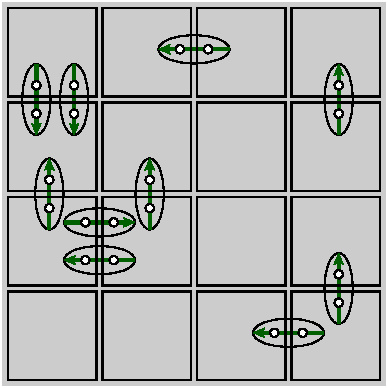
\includegraphics[width=0.3\columnwidth ]{pic-pair-create.pdf}
\end{center}
Each such pair will have vacuum total charge and so the observables
$\gamma_{ij}$ will only see pairs that intersect, ie. we
need only consider distributing these pairs
transversally along edges of the tiles.

In order to compute measurement outcomes for the $\gamma_{ij}$
we first need to concatenate any two curve diagrams that 
participate in the same $\gamma_{ij}.$
Because each curve has vacuum total charge this can be
done in an arbitrary way:
\begin{center}
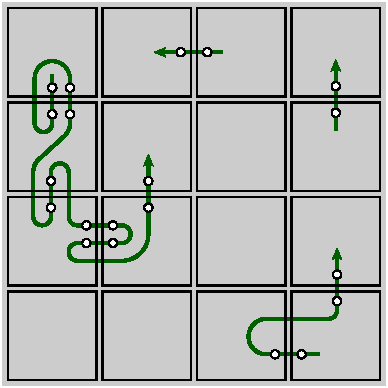
\includegraphics[width=0.3\columnwidth ]{pic-join-pairs.pdf}
\end{center}

Working in the basis picked out by the resulting curve
diagrams, we can calculate measurement probabilities for each tile.
The measurement outcomes are then randomly sampled,
and the results recorded on the original curve:
\begin{center}
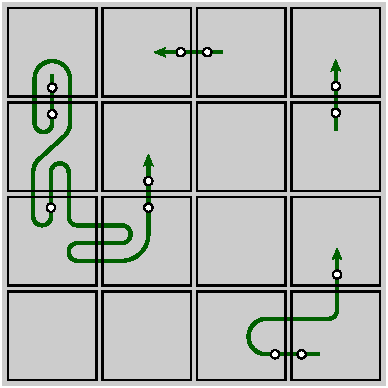
\includegraphics[width=0.3\columnwidth ]{pic-curve-uniq.pdf}
\end{center}
%\cggb{It might be helpful to be a bit more explicit either here or later about exactly how we perform this step, moving charges around with the paperclip algorithm until they are all neighbouring and then we are in a standard basis and can use F-moves to calculate fusion outcomes.}
%\simon{good idea}

%\danbrowne{Have you explained this measurement rule anywhere? In particular, how is the outcome of the measurement derived from the curve? Is this measurement deterministic or non-deterministic?}

As another example of the kind of calculation that needs to be performed,
here we zoom-in and show an example involving just two tiles (inside a larger tiling):
\begin{center}
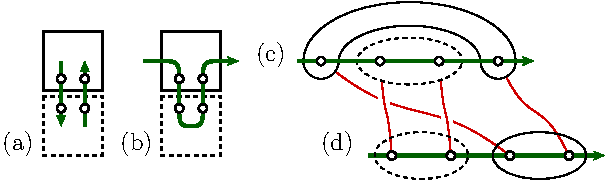
\includegraphics[width=0.8\columnwidth]{pic-syndrome.pdf}
\end{center}
In (a) we have two pair-creation events, each crossing the boundary of a tile. 
One observable (tile) is solid black, and the other observable is dashed.
The problem we solve here is that 
these observables are different from the observables making up the
pair-creation events.
In (b) we join the participating curve 
diagrams arbitrarily into a single curve diagram.
%This could already become very complicated, even if we
%stick to these two tiles
The curve diagram (c) is the same as (b), we just
pulled the curve straight (an isotopy).
%The total charge of each tile can then be found 
Now we braid anyons around each other until all charges within 
a tile are neighbors on the curve, as in (d).  
%\footnote{This is a standard POP decomposition, see section 3.3.}
The red lines then correspond to the worldlines for these braids.
The state (d) is equivalent to the original
state (a), but now the observables we need (the solid and dashed
black lines) are at most a few $F-$moves away.

If the reader finds this confusing, that's because it \emph{is}
confusing. This is why so much care and detail was taken in chapter 3.
The systematic implementation of these calculations relies on all the
machinery developed in chapter 3, in particular the refactoring theorem of
section 3.4.
%We have yet to describe the details of this is implementation:
The data structure we will use is called a \emph{combinatorial curve diagram}
and is described in section 4.4.1.
The algorithm that operates on this data is called the 
\emph{paper-clip algorithm} and will be described in section 4.4.2.
This data structure and algorithm is a combinatorial version of the theory
of modular functors suitable for implementation on a classical computer.

We consider this treatment of anyon dynamics to be a phenomenological model in that
it neglects any microscopic details of the system.
This is consistent with the principles of topologically
ordered systems and anyonic physics, where the key universal features describing the
anyon model correspond to large length-scale physics, while the microscopic physics plays
a less important (and non-universal) role. Note also that our analysis applies equally well to either a continuum setting, or to discrete lattice models supporting anyonic excitations.
%Additionally, while we model a continuum anyon theory, our analysis can be trivially reinterpreted to apply directly to lattice spin models or other systems where space is fundamentally discrete.

In order to perform a logical error on our code, a noise process must have support on a
a region of the manifold that is non-local, (cannot be contracted).
%\danbrowne{Why does homology play a role here? Don't forget to introduce the logical operators of this qubit. }
These correspond to processes in which anyonic charge is transported around a non-trivial loop before annihilating to vacuum.
We do not consider these processes as we regard the decoding
to have failed if any such non-local process would occur.



%
% ~~~~~~~~~~~~~~~~~~~~~~~~~~~~~~~~~~~~~~~~~~~~~~~~~~~~~~~~~~~~~~~~~~~~~~~~~~~~
%

\section{Decoding algorithm}

After the noise process is applied to the system,
the error correction proceeds as a dialogue between the
decoder and the system. 
In this section we describe the decoder side of this dialogue,
the quantum side is much more difficult and is discussed in the
following sections.
%
%Our error-correction algorithm begins by measuring the charge on
%each tile of the lattice, producing a \emph{syndrome}
%of occupied sites. Following this, it joins nearby
%occupied tiles into clusters, and measures the total charge within each cluster.
%Clusters with trivial charge are
%discarded, and then nearby clusters
%are merged (agglomeratively~\cite{Hastie2009}).
%The merging process iterates at
%linearly increasing length scales, at
%each step measuring total charge
%and discarding trivial clusters, before concluding when
%there is at most a single cluster remaining (see \Fref{f:decode}).
%
%
The decoder measures succesively larger and larger
regions of the lattice
until there are no more charges 
or a topologically non-trivial operation has occured
(an operation that spans the entire lattice.)
In Figure \ref{PicProcess}
we show this in a process diagram, with time running up
the page.
Note that unlike the case of abelian anyons, the decoder
cannot determine the charge of each cluster 
given only the syndrome information (as in Ref. \cite{Bravyi2011}),
and so must repeatedly physically query the system to measure these charges.




%\begin{samepage}
\begin{figure}
\begin{verbatim}
 1:  def decode():
 2:      syndrome = get_syndrome()
 3:      
 4:      # build a cluster for each charge
 5:      clusters = [Cluster(charge) for charge in syndrome]
 6:  
 7:      # join any neighbouring clusters
 8:      join(clusters, 1)
 9:      
10:      while clusters:
11:      
12:          # find total charge on each cluster
13:          for cluster in clusters:
14:              fuse_cluster(cluster)
15:      
16:          # discard vacuum clusters
17:          clusters = [cluster for cluster in clusters if non_vacuum(cluster)]
18:      
19:          # grow each cluster by 1 unit
20:          for cluster in clusters:
21:              grow_cluster(cluster, 1)
22:      
23:          # join any intersecting clusters
24:          join(clusters, 0)
25:  
26:      # success !
27:      return True
\end{verbatim} % see decode.py
%\end{samepage}
\caption{Pseudo-code listing for the (classical) decoding algorithm.}
\label{PseudoCode}
\end{figure}

%So far we have discussed the simulation of the (quantum) system
%and now we turn to the decoder algorithm.
In Figure \ref{PseudoCode} we show a pseudo-code listing for the
decoder algorithm,
and we explain each step via an example below.
This decoder is based on
a hierarchical clustering algorithm~\cite{Hastie2009, Wootton2015b},
and follows a similar strategy to
the hard-decision renormalization group decoder~\cite{Bravyi2011}.

\begin{samepage}
First, we show the result of the initial call to {\tt get\_syndrome()}, on line 2.
The locations of anyon charges are indicated by the thick black circles.
For each of these charges we build a {\tt Cluster}, on line 5.
Each cluster is shown as a gray shaded area in the following diagrams.
\begin{center}
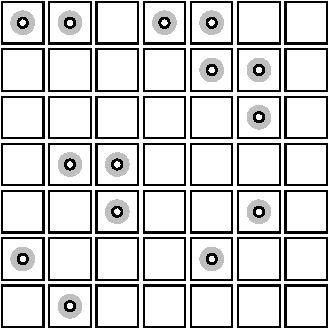
\includegraphics[]{pic-decode-0.pdf}
\end{center}
\end{samepage}

\begin{samepage}
The next step is the call to {\tt join(clusters, 1)}, on line 8,
which joins clusters that are separated by at most one lattice
spacing. We now have seven clusters:
\begin{center}
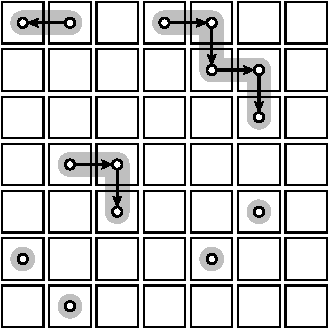
\includegraphics[]{pic-decode-1.pdf}
\end{center}
\end{samepage}

Each cluster is structured as a rooted tree, as indicated by
the arrows which point in the direction from the leaves to
the root of the tree. 
This tree structure is used in the call to {\tt fuse\_cluster()},
on line 14.
This moves anyons in the tree along the arrows to the root, 
fusing with the charge at the root.
\begin{center}
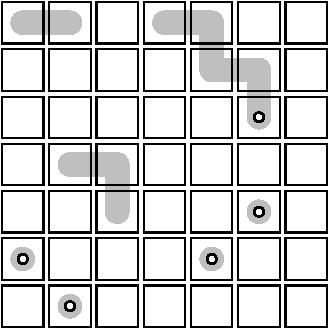
\includegraphics[]{pic-decode-2.pdf}
\end{center}

For each cluster, the resulting charge at the root is taken as the charge of
that cluster. Any cluster with vacuum total charge is then discarded (line 17).
%In our example, we assume all these charges are non-vacuum.
In our example, we find two clusters with vacuum charge and we discard these.
The next step is to grow the remaining clusters by one lattice spacing (line 20-21),
and join (merge) any overlapping clusters (line 24).
\begin{center}
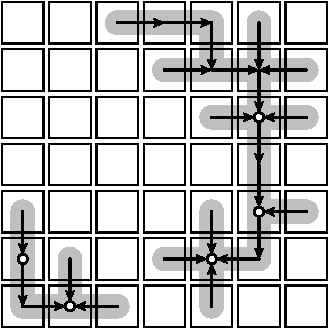
\includegraphics[]{pic-decode-3.pdf}
\end{center}

%Now we are down to two clusters.
Note that we can choose the root of each cluster arbitrarily,
as we are only interested in the total charge of each cluster.

We repeat these steps of fusing, growing and then joining clusters (lines 10-24.)
If at any point this causes a topologically 
non-trivial operation, the simulation aborts and a failure
to decode is recorded.
Otherwise we eventually run out
of non-vacuum clusters, and the decoder succeeds (line 27).
For simplicity we have neglected the boundary of the lattice in
this example.


%
% ~~~~~~~~~~~~~~~~~~~~~~~~~~~~~~~~~~~~~~~~~~~~~~~~~~~~~~~~~~~~~~~~~~~~~~~~~~~~
%

\section{Simulation of the quantum system}

It is known that the process of braiding and fusing
Fibonacci anyons is sufficient to implement universal quantum
computing, so at first sight it seems foolish to try to simulate
this using classical computers. % \cite{Freedman2002, Nayak2008|

However, it turns out to indeed be possible, up to some reasonably
large system sizes. 
The reasons why are outlined in a heuristic manner as follows.
The decoding threshold (see Figure \ref{AnyonsKyle})
occurs far below the bond percolation threshold.
Below this percolation threshold, error processes 
decompose into separate components of
average size $O(\log(L))$ and variance $O(1)$~\cite{Bazant2000}.
Each such component can be simulated separately, ie.
each component corresponds to a tensor factor of the
Hilbert space of the system 
(this is the monoidal axiom, Section \ref{ModularFunctors}).
Because the average size of such a component
is $O(\log(L))$ the corresponding fusion space will have 
dimension $O(\mathrm{poly}(L)).$

Working against this system separability is the
action of the decoder, which will tend to join (fuse)
nearby anyons and thereby also at times connect separate
components. 
All is not lost, however, as this act of fusing also
reduces the number of anyons needed to be simulated.

At some point, with high enough error rate, the combined action of
noise plus decoder will become exponentially difficult to simulate.
Nevertheless, we are able to simulate error-correction in
the regime around the error-correction threshold for linear lattice sizes up to $L=128$.
See Figure \ref{AnyonsKyle} below.

We now turn to a description of the data-structures and algorithm
used to simulate the quantum system.
This relies heavily on the theory developed in Chapter 3.

%
% ~~~~~~~~~~~~~~~~~~~~~~~~~~~~~~~~~~~~~~~~~~~~~~~~~~~~~~~~~~~~~~~~~~~~~~~~~~~~
%

\subsection{Combinatorial curve diagrams}

The basic data structure involved in the
simulation of the quantum system
we term a \emph{combinatorial curve diagram.}
This is essentially a combinatorial formulation of the
theory of modular functors presented in Chapter 3.
The sole purpose of this formulation is to
be able to simulate fusion outcomes for each of the observables in the
lattice $\Lambda := \bigl\{ \gamma_{ij} \bigr\}_{i,j=1,...,L}.$
For each tile in this lattice,
we store a combinatorial
description of the curve(s) intersected with that tile.
\begin{center}
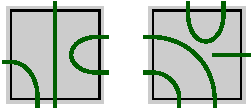
\includegraphics[]{pic-cells.pdf}
\end{center}
Each component of such an intersection we call a \emph{piece-of-curve.}
We follow essentially the same approach as taken in Ref.~\cite{Abramsky2007} 
to describe elements of a Temperley-Leib algebra, but
with some extra decorations.
Firstly, we will require each curve to intersect 
the edges of tiles transversally,
and in particular a curve will not touch a tile corner.
The key idea is to store a \emph{word} for each tile, comprised of
the letters $\bigl<$ and $\bigr>$.
%The encoding works as follows.
Reading in a clockwise direction around the edge of
the tile from the top-left corner,
we record our encounters with each piece-of-curve,
writing~$\bigl<$ for the first encounter, and~$\bigr>$ for the
second.
We may also encounter a dangling piece-of-curve
(the head or the tail), so we use another symbol $*$ for this.
The words for the above two tiles will then be 
$\bigl<\bigl<\bigr>\bigr>\bigl<\bigr>$ and $\bigl<\bigr>*\bigl<\bigl<\bigr>\bigr>.$
When the brackets are balanced,
each such word will correspond one-to-one with an intersection
of a curve in a tile, up to a continuous deformation of the interior of the tile.
Ie. the data structure 
will be insensitive to any continuous deformation of the interior of the tile,
but the simulation does not need to track any of these degrees of freedom.

\begin{center}
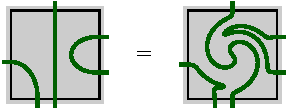
\includegraphics[]{pic-cells-0.pdf}
\end{center}

We will also need to record
various other attributes of these curves,
and to do this we make this notation more elaborate
in the paragraphs {\bf (I)}, {\bf(II)} and {\bf(III)} below.
Each symbol in the word describes an intersection of
the curve with the tile boundary,
and so as we decorate these symbols these decorations will
apply to such intersection points.

\begin{center}
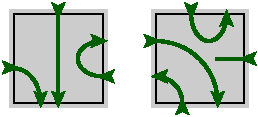
\includegraphics[]{pic-cells-1.pdf}
\end{center}

{\bf (I)} We will record the direction of each piece-of-curve,
this will be either an {\tt in} or {\tt out} decoration for each symbol.
Such decorations need to balance according to the brackets.
The decorated symbols $*_{\mathrm{\tt in}}$ and 
$*_{\mathrm{\tt out}}$ 
will denote respectively either
%the head, $c(1)$ or the tail $c(0)$ of a curve.
the head or the tail of a curve.
The words for the diagrams above now read as
$ \bigl<_{\mathrm{\tt in}}\bigl<_{\mathrm{\tt out}}\bigr>_{\mathrm{\tt in}}
    \bigr>_{\mathrm{\tt out}}\bigl<_{\mathrm{\tt out}}\bigr>_{\mathrm{\tt in}}$
and
$ \bigl<_{\mathrm{\tt in}}\bigl>_{\mathrm{\tt out}}*_{\mathrm{\tt in}}
    \bigr<_{\mathrm{\tt out}}
    \bigr<_{\mathrm{\tt in}}\bigl>_{\mathrm{\tt out}}\bigr>_{\mathrm{\tt in}}.
$

\vskip 10pt
{\bf (II)} We will record,
for each intersection with the tile edge, 
a numeral indicating which of the four
sides of the tile the
intersection occurs on.
Numbering these clockwise from the top as $1, 2, 3, 4$ we have for the above curves: 
$\bigl<_1\bigl<_2\bigr>_2\bigr>_3\bigl<_3\bigr>_4$ 
and $\bigl<_1\bigr>_1*_2\bigl<_3\bigl<_3\bigr>_4\bigr>_4.$

\vskip 10pt
{\bf (III)} Finally, we will also decorate these symbols with anyons.
This will be an index to a leaf of a (sum of) fusion tree(s).
This means that anyons only reside on the curve close
to the tile boundary,
and so we cannot have more than two anyons
for each piece-of-curve. 
The number of such pieces is arbitrary, and so this
is no restriction on generality.

\begin{center}
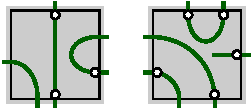
\includegraphics[]{pic-cells-2.pdf}
\end{center}

In joining tiles together to make a tiling we will
require adjacent tiles to agree on their shared boundary.
This will entail sequentially pairing symbols in the
words for adjacent tiles
and requiring that 
the {\tt in} and {\tt out} decorations are matched.
Because the word for a tile proceeds counter-clockwise
around the tile, this pairing will always reverse the
sequential order of the symbols of adjacent tiles.
For example, given the above two tiles we sequentially pair the 
$\bigl<_{\mathrm{\tt out},2}\bigr>_{\mathrm{\tt in},2}$ 
and $\bigr>_{\mathrm{\tt out},4}\bigr>_{\mathrm{\tt in},4}$
symbols with opposite order so that
$\bigl<_{\mathrm{\tt out},2}\sim\bigr>_{\mathrm{\tt in},4}$
and $\bigr>_{\mathrm{\tt in},2} \sim \bigr>_{\mathrm{\tt out},4}.$ 

\vskip 5pt

%Two other consistency relations are enforced on such a combinatorial curve diagram:
%we require adjacent tiles to agree on their boundaries, 
%and every curve diagram
%must have two ends.
%One final consistency
%relation is enforced by requiring 
%We require every curve diagram to have two ends, this means
%that there are no loops.

Note that in general this data structure will store many disjoint curve diagrams
$c_i:[0,1]\to D_{n_i}$ within a disc $D_m$ where $\sum n_i = m.$

%For a given piece-of-curve, we can subtract the numeral with
%the {\tt in} label from the numeral with the {\tt out} label
%to get an integer in $\{ \}$ WRONG
%We can also just use the numerals of the boundary edges
%that the piece-of-curve intersects with, subtracting the
%``exit'' boundary numeral from the ``entry'' boundary numeral. WRONG

For each piece-of-curve, apart from a head or tail, there is an associated 
number we call the \emph{turn number}. This counts the number
of ``right-hand turns'' the piece-of-curve makes as it
traverses the tile, with a ``left-hand turn'' counting as $-1.$
(To be more rigorous, we would define this number using the
winding number of the simple closed curve formed by the
piece-of-curve adjoined to a segment of the boundary of the tile 
traversed in a clockwise direction.)
This number will take one of the values $-2, -1, 0, 1, 2:$
\begin{center}
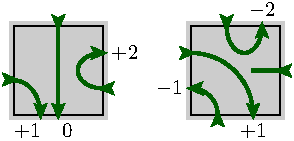
\includegraphics[]{pic-cells-3.pdf}
\end{center}


%Two disjoint curves can be joined by...
%
%Curves can be simplified along sections without any anyons, ...

% Each piece will have +1, +2, 0, -1, -2 right-hand turns...

% mention Jones' planar algebras ?

%
% ~~~~~~~~~~~~~~~~~~~~~~~~~~~~~~~~~~~~~~~~~~~~~~~~~~~~~~~~~~~~~~~~~~~~~~~~~~~~
%

\subsection{The paperclip algorithm}

In the description of the refactoring theorem
in Section \ref{RefactoringTheorem}
we thought of $R$-moves as acting on the basis of
the system as in the Heisenberg picture.
Now we switch to an equivalent perspective and
consider $R$-moves as transport of anyon charges
as in a Schrodinger picture.
The anyons will be transported around the lattice
by moving them along tile edges.
%\simon{Note that transport here is the same as the refactoring from above.}
In general, such a transport will intersect with a
curve diagram in many places.
Each such intersection is transverse,
and we use each intersection point to cut
the entire transport into smaller paths each of
which touch the curve diagram twice.
%Each intersection with a curve diagram
%will then be transverse, and we
%decompose the entire path into a sequence of
%paths each of which 
%join consecutive intersections.
%Transport of an anyon can be decomposed into
%moves between adjacent components of a curve
%diagram.
The origin and destination of such an anyon path
now splits the curve diagram $c:[0, 1]\to D_n$ 
into three disjoint pieces which we term
\emph{head}, \emph{body} and \emph{tail}, where
the head contains the point $c(1)$, the tail
contains $c(0)$ and the body is the third piece.
These arise with various arrangements, but here
we focus on one instructive case, the
other cases are similar:
%We look at the particular case of moving along
%one edge of a tile,
transporting along one edge of a tile \emph{forwards} 
(from tail to head) along a curve diagram:
\begin{center}
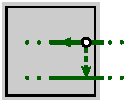
\includegraphics[]{pic-move-anyon.pdf}
\end{center}

This arrangement is equivalent (isotopic) to one of four 
``paperclips'', which we distinguish between by counting how
many \emph{right-hand turns} are made along the body of the curve diagram.
We also show an equivalent (isotopic) picture where the
curve diagram has been straightened, and the resulting distortion
in the anyon path:
\begin{center}
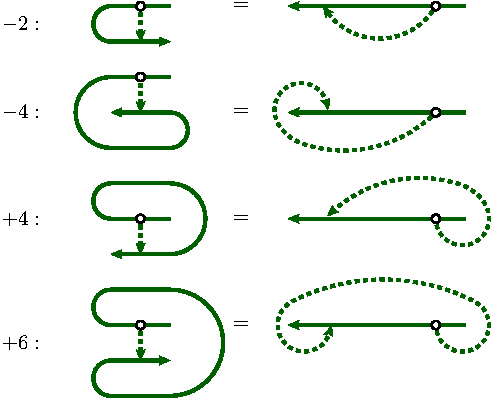
\includegraphics[]{pic-paperclip.pdf}
\end{center}
The sequence of anyons along the head, body and tail, we denote as $H, B$ and $T,$
respectively.
These sequences have the same order as the underlying curve diagram, and 
we use
$H^r, B^r$ and $T^r$ to denote the same anyons with the reversed order.
Using the above diagram, we can now read off the $R$-moves for each
of the four paperclips:
\begin{align*}
-2:&\ R[B] \\
-4:&\ R[H^r]\ R[H]\ R[B] \\
+4:&\ R[B]\ R[T]\ R[T^r] \\
+6:&\ R[H^r]\ R[H]\ R[B]\ R[T]\ R[T^r] \\
\end{align*}
where notation such as $R[B]$ is understood as sequentially clockwise braiding around
each anyon in $B$.

That these four paperclips exhaust all possibilities can be seen by
considering the winding number of the simple closed curve made
by combining the body of the curve diagram with the path followed by
the anyon (appropriately reversing direction as needed).

\section{Numerical results}


\begin{figure}
\begin{center}
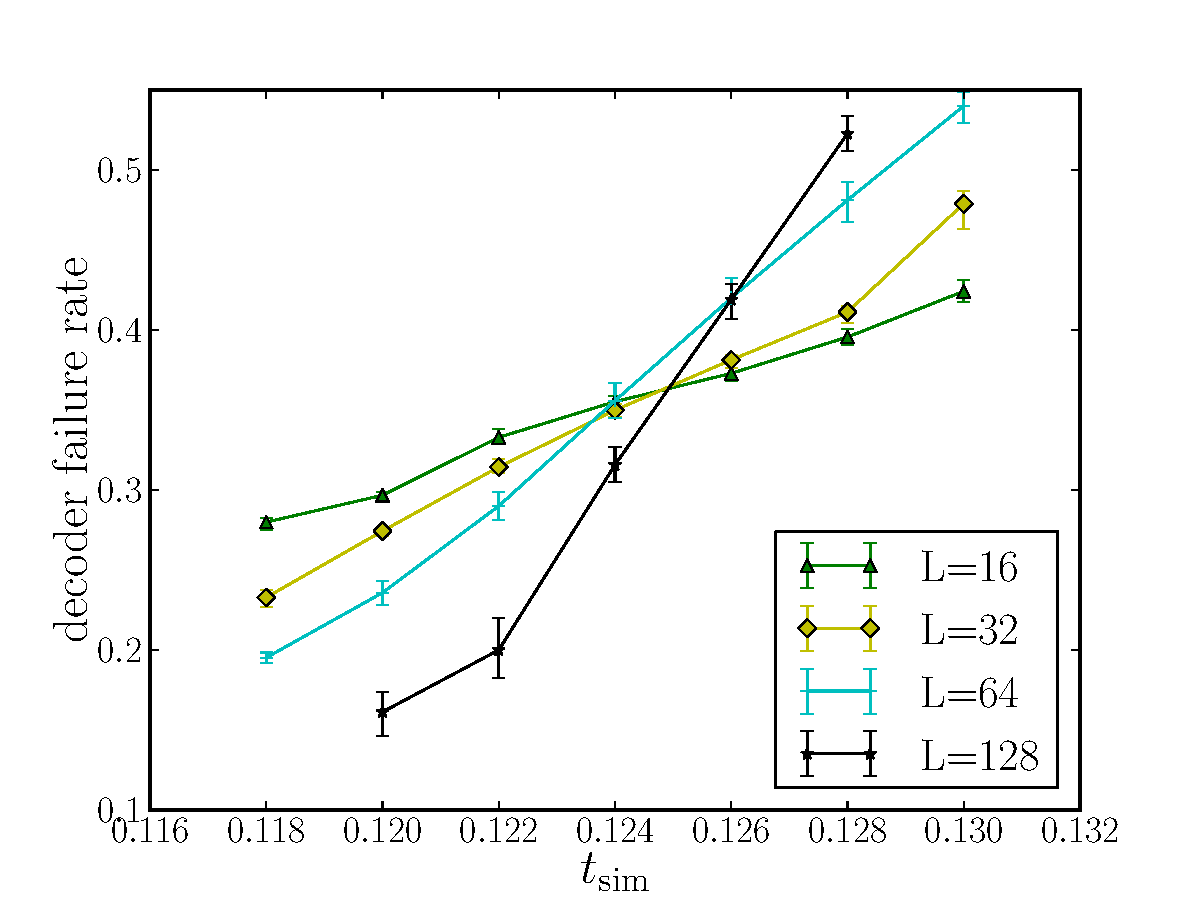
\includegraphics[width=0.8\columnwidth]{anyons-kyle.pdf}
\caption{
Results of monte-carlo sampling of the decoding simulation for
various lattice sizes $L$ and expected pair-creation events per
edge $t_{\mathrm{sim}}.$
}
\label{AnyonsKyle}
\end{center}
\end{figure}

The results of simulating the noise plus decoder are shown in
Figure \ref{AnyonsKyle}.
We run a monte-carlo simulation, for various lattice sizes $L$,
and error rate per edge $t_{\mathrm{sim}}.$
The number of pair-creation
processes accross each edge of the lattice
is sampled from a Poisson process,
and $t_{\mathrm{sim}}$ indicates the expected value of this 
Poisson process.

The decoder failure rate shows a clear threshold at around 
$t_{\mathrm{sim}}=0.125\pm0.003.$ 
Below this threshold errors are increasingly suppressed 
as the lattice size grows.

%The appearance of this threshold is perhaps not surprising as
%the underlying processes resemble a kind of percolation problem.
%\todo{XXX}

%\section{Computation of homologically non-trivial operators}\label{s:homnontrivial}
%
%Specializing to the Fibonacci case,
%we write the non-trivial $F$-moves as the following
%skein relations:
%\begin{align*}
%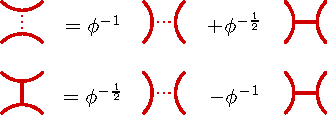
\includegraphics[]{pic-skein1.pdf}
%\end{align*}
%
%The sollid lines represent Fibonacci world-lines.
%The dotted lines represent vacuum charges,
%and we are free to include these lines or not.
%We leave these anyon paths
%as undirected because Fibonacci anyons are
%self-inverse.
%The non-trivial $R$-moves are:
%\begin{align*}
%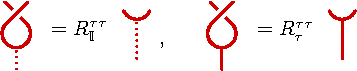
\includegraphics[]{pic-skein2.pdf}
%\end{align*}
%
%Removing bubbles:
%\begin{align*}
%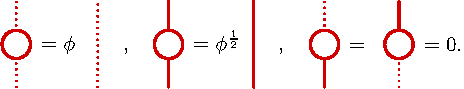
\includegraphics[]{pic-bubble.pdf}
%\end{align*}
%
%Here we show a process where a 
%Fibonacci anyon travels around the torus and
%anihilates itself. Twice.
%The vertical lines represent a periodic
%identification.
%\begin{align*}
%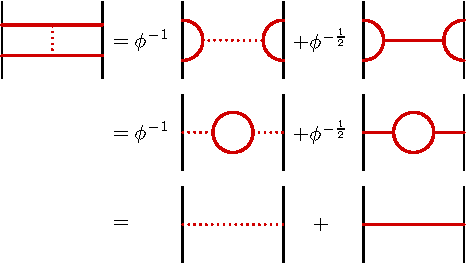
\includegraphics[]{pic-logops.pdf}
%\end{align*}
%
%The state is not normalized.
%Also involves post-selection, as there is
%another process that involves leakage...
%The first equation is an $F$-move, 
%the second equation is a translation in the
%horizontal direction, and the last equation
%follows from the rule for collapsing bubbles.
%
%Continuing in this way, we compute the $k$-fold
%logical operator:
%\begin{align*}
%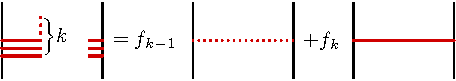
\includegraphics[]{pic-kfold.pdf}
%\end{align*}
%
%where $f_k$ is the $k$-th element of the Fibonacci
%sequence $\{1, 1, 2, 3...\}.$


\section{Discussion}

In this chapter we simulated a non-abelian anyon system acting as
a quantum error correcting code.

The algorithms for simulating non-abelian anyons in general require
the machinery of modular functors which was described in Chapter 3.
We reformulated this theory in a combinatorial way suitable for
simulation on a classical computer.

Because the anyons involved are universal for quantum computing it
would at first sight appear to be too difficult to simulate,
but we are able to succeed anyway by decomposing the system into smaller
non-interacting parts. This turns out to work 
sufficiently well in the regime of interest, where there are
few anyons widely separated.

We use a standard error correction algorithm that involves
clustering together nearby anyons, and fusing these until there
are no anyons remaining.

We present numerical evidence of threshold behaviour:
below a certain noise rate, the code error rate decreases as
the system size grows.

The simulation algorithms used here
would apply to any other anyon system by merely replacing
the $F$ and $R$ matrices.
Higher genus surfaces could also be simulated, these would store
more qubits, but would involve a more complicated tiling structure.

Quantum information can also be stored in the fusion space of
four widely separated anyons, but this may be computationally
harder to simulate
as the system does not decompose into non-interacting parts in an
obvious way as above.

%It is not so clear how to simulate a
%It would seem likely
%that similar threshold numerics would be obtained.



